% LaTeX Template for Project Report, Version 2.0
% (Abstracted from a Major Project Report at CSED, NIT Calicut but can be
% modified easily to use for other reports also.)
%
% Released under Creative Commons Attribution license (CC-BY)
% Info: http://creativecommons.org/licenses/by/3.0/
%
% Created by: Kartik Singhal
% BTech CSE Batch of 2009-13
% NIT Calicut
% Contact Info: kartiksinghal@gmail.com
%
% It is advisable to learn the basics of LaTeX before using this template.
% A good resource to start with is http://en.wikibooks.org/wiki/LaTeX/
%
% All template fields are marked with a pair of angular brackets e.g. <title here>
% except for the ones defining citation names in ref.tex.
%
% Empty space after chapter/section/subsection titles can be used to insert text.
%
% Just compile this file using pdflatex after making all required changes.

\documentclass[12pt,a4paper]{report}
\usepackage[pdftex]{graphicx} %for embedding images
\usepackage{url} %for proper url entries
\usepackage[bookmarks, colorlinks=false, pdfborder={0 0 0}, pdftitle={<pdf title here>}, pdfauthor={<author's name here>}, pdfsubject={<subject here>}, pdfkeywords={<keywords here>}]{hyperref} %for creating links in the pdf version and other additional pdf attributes, no effect on the printed document
%\usepackage[final]{pdfpages} %for embedding another pdf, remove if not required

\begin{document}
\renewcommand\bibname{References} %Renames "Bibliography" to "References" on ref page

%include other pages
\begin{titlepage}

       \begin{center}
       
       \textup{\small {\bf CS6100 Course Project} \\ Report}\\[0.2in]
       
       % Title
       \Large \textbf {Chriostofides' Short-cutting heuristics for Euclidean metric Travelling salesman problem}\\[0.5in]
       
              \small \emph{Submitted in partial fulfillment of\\
               the requirements for the award of the degree of}
               \vspace{.2in}
       
              {\bf Bachelor of Technology \\in\\ Computer Science and Engineering}\\[0.5in]
       
       % Submitted by
       \normalsize Submitted by \\
       \begin{table}[h]
       \centering
       \begin{tabular}{lr}\hline \\
       Roll No & Names of Students \\ \\ \hline
       \\
       CS17B005 & A. Subhash \\
       CS17B011 &  D. Varun Teja\\
       CS17B012 &  D.M.S Krishna\\
       CS17B021 &  P. Jaitesh\\\hline 
       \end{tabular}
       \end{table}
       
       \vspace{.1in}
       Under the guidance of\\
       {\textbf{Prof. B. V. Raghavendra Rao}}\\[0.2in]
       
       \vfill
       
       % Bottom of the page
       % 
\includegraphics[width=0.18\textwidth]{./nitc-logo}\\[0.1in]
       \Large{Department of Computer Science and Engineering}\\
       \normalsize
       \textsc{IIT Madras}\\
       % Chennai \\
       % \vspace{0.2cm}
       % Winter Semester 2013
       
       \end{center}
       
       \end{titlepage}
       
% \newpage
\thispagestyle{empty}

\begin{center}

\huge{Department of Computer Science and Engineering}\\[0.5cm]
\normalsize
\textsc{National Institute of Technology Calicut}\\[2.0cm]

\emph{\LARGE Certificate}\\[2.5cm]
\end{center}
\normalsize This is to certify that this is a bonafide record of the project presented by the students whose names are given below during <Monsoon/Winter and Year here> in partial fulfilment of the requirements of the degree of Bachelor of Technology in Computer Science and Engineering.\\[1.0cm]

\begin{table}[h]
\centering
\begin{tabular}{lr}
Roll No & Names of Students \\ \\ \hline
\\
<Roll no here> & <Name here> \\ 
<Roll no here> & <Name here> \\
<Roll no here> & <Name here> \\
\end{tabular}
\end{table}

\vfill


% Bottom of the page
\begin{flushright}
<Guide name here>\\
(Project Guide)\\[1.5cm]
<Coordinator name here>\\
(Course Coordinator)\\
\end{flushright}

\begin{flushleft}
Date:
\end{flushleft}

\vspace{2in}
\begin{abstract}
Several $O(n), O(n^2)$ short-cutting heuristics are described which are used in Christofides' algorithm for solving n-city travelling salesman problems whose cost matrix satisfies the triangularity condition. The Christofides' algorithm invovles computation of a shortest spanning tree of the graph G defining the TSP, and finding the minimum cost perfect matching of a certaing induced subgraph of G. 
\end{abstract} 


\pagenumbering{roman} %numbering before main content starts
\tableofcontents
\listoffigures

\newpage
\pagenumbering{arabic} %reset numbering to normal for the main content

\chapter{Problem Definition}

The goal is to find more efficient(in terms of solution cost) short-cutting heuristics which are used in the last step of Christofides' algorithm for finding the TSP tour.

 %objective changed to problem definition
\chapter{Introduction}

\section{Metric space}

A metric $d$ on a set $X$, also called a distance function, is a function
that defines a distance between each pair of elements of the set. A
set with a metric is called a \textbf{metric space}.\\

Formally, $d : X \times X \rightarrow R$ is a metric if it is a function satisfying the following properties $\forall x, y, z \epsilon X$:
\begin{enumerate}
\item{Non-negativity : $d(x, y) \geq 0$}
\item{Indiscernability : $d(x, y) = 0$ iff $x = y$}
\item{Symmetry : $d(x, y) = d(y, x)$}
\item{Subadditivity : $d(x, y) + d(y, z) \geq d(x, z)$}
\end{enumerate}
\section{The Christofides' algorithm}
The Christofides' algorithm is an approximation algorithm for Metric TSP with an approximation ratio of $1.5$. Let G be a graph with $n$ points in the euclidean metric space. Below is a description of the steps involved in the Christofides' algorithm.
\vspace{0.7in}
\subsection{Pseudo code}
\textbf{Algorithm}
\begin{enumerate}
    \item{
        Find an MST of $G$, say $T$.        
    }
    \item {Compute a minimum cost perfect matching, $M$, on the set of odd-degree vertices of $T$.}
    \item {
        Add $M$ to $T$ and obtain an Eulerian multi-graph $H$.
    }
    \item {Find an Euler tour, $E$ of this graph.
    }
    \item {Output the tour that visits vertices of $G$ in order of their first appearance in $E$.}
\end{enumerate}
\begin{figure}[h]
    \centering
    \caption{MST $T$ of $G$}
    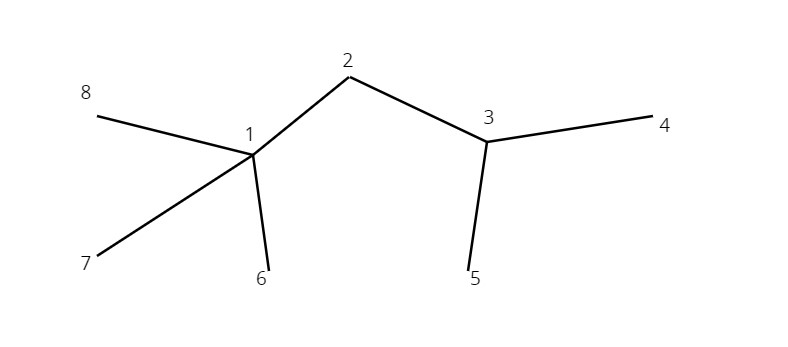
\includegraphics[scale=0.3]{1.jpg}
\end{figure}        
\begin{figure}[h]
    \centering
    \caption{Multi-graph $H$ of $G$}
    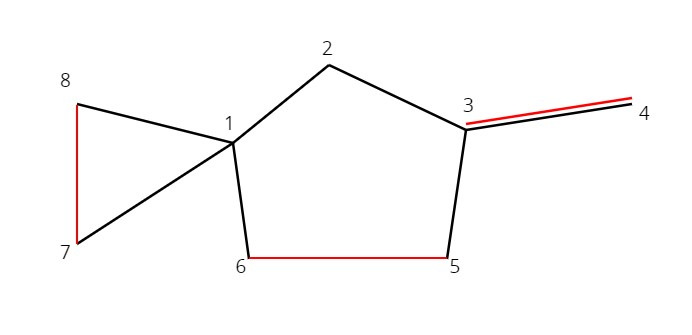
\includegraphics[scale=0.3]{2.jpg}
\end{figure}
\begin{figure}[h]
    \centering
    \caption{Euler tour $E$ of $H$}
    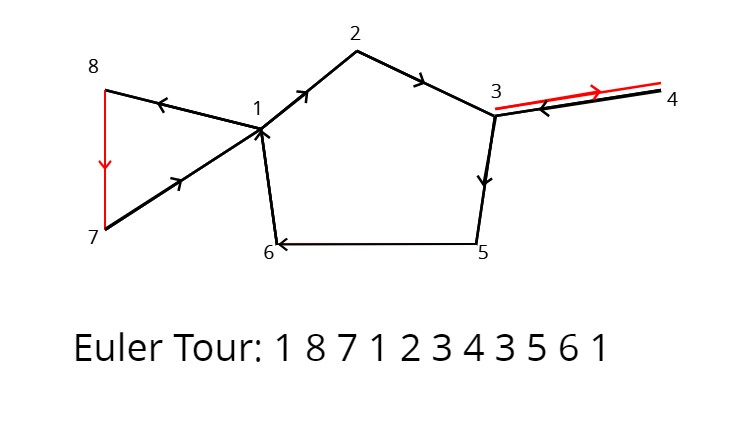
\includegraphics[scale=0.3]{3.jpg}
\end{figure}
\subsection{Time complexity}
\begin{enumerate}
    \item {Creating MST $T$ of $G$ : $O(nlogn)$}
    \item {Finding the minimum cost perfect matching $M$ : $O(n^3)$}
    \item {Creating multi-graph H : $O(n)$}
    \item {Finding Euler tour $E$ in $H$ : $O(n)$}
\end{enumerate}
% some text\cite{citation-1-name-here}, some more texts
% even more text\footnote{<footnote here>}, and even more.
% \section{Motivation}
 %literature survey included in this
\chapter{Short-cutting heuristics}


\section{Simple Heuristic}
\begin{enumerate}
    \item Remove repeated points in the Euler tour to get a Hamiltonian cycle.
    \item Time complexity is $O(n)$
\end{enumerate}
% \includegraphics[scale=0.5]{simple.png}

\section{Tri-Opt Heuristic}

\begin{enumerate}
    \item In this hurestic we take a Euler tour and greedily remove the repeated vertices
    \item The hurestic value used is sum of distances from the vertex to adjacent vertices minus distance between the adjacent vertices
    \item We can see that this is better than previous one but we are performing it on a Euler tour, hence there is still room for imprevement
    \item Time complexity is $O(n)$
\end{enumerate}
% \includegraphics[scale=0.5]{simple.png}



\section{Tri-Comp Heuristic}

\begin{enumerate}
    \item This hurestic is applied on Multi graph (H) instead of one Euler tour
    \item Here we start with vertices of order greater than two and greedily remove its edges until its order is two
    \item The idea is that in the final hamiltonian cycle which we need to arrive by short cutting has degree two for all the vertices
    \item Two things we need to do are - pair up the free vertices formed greedily and make sure the process does not result in two disjoint components
    \item The hurestic value here is sum of distances between paired up vertices and distace of two edges that remained with our vertex
    \item Since our problem is in 2d space, each vertex in MST will have a degree of maximum 5, so our multi graph will have a maximum degree of 6. This property highly affect the theoritical complexity of our hurestic
    \item Time complexity for checking the graph connectivity is $O(n)$ and for complete hurestic is $O(n^2)$
\end{enumerate}
% \includegraphics[scale=0.5]{simple.png}

\section{DIH-Tri-Comp Heuristic}

\begin{enumerate}
    \item This hurestic is DIH(Degree Increasing Heuristic) optimization applied on the previous one
    \item We want to increase the order of a vertex in MST by adding the vertices  of its children to itself
    \item We can see that the tree is no longer MST but this process preserves the Euler tours i.e. the set of Euler tours of this tree is super set of that of the MST
    \item This way we are applying hurestic on bigger space than that of the former one and have a chance of getting better results
    \item  DIH can be implemented with $O(n)$, so comp hurestic is the bottleneck here. Overall complexity is $O(n^2)$
\end{enumerate}
% \includegraphics[scale=0.5]{simple.png}




% Refer figure \ref{fig:label}

% \begin{figure}[htb]
% \centering
% 
\includegraphics[scale=0.3]{./glider} % e.g. insert ./image for image.png in the working directory, adjust scale as necessary
% \caption{<Caption here>}
% \label{fig:label} % insert suitable label, this is used to refer to a fig from within the text as shown above
% \end{figure}

% \subsection{<Sub-section title>}


% \section{<Section title>}


\chapter{Future Work}

<Future work here>

\chapter{Conclusion}

<Conclusion here>

\cleardoublepage
%\pagebreak
\phantomsection
\addcontentsline{toc}{chapter}{Acknowledgements}
\chapter*{Acknowledgments}
\vspace{1.0in}
<Acknowledgements here>
\\
\\
\\ 
\\
<Name here> \\ 
\\
<Month and Year here>\\
{National Institute of Technology Calicut}\\
\newpage

\cleardoublepage
%\pagebreak
\phantomsection
\addcontentsline{toc}{chapter}{References}
\begin{thebibliography}{99}

\bibitem{citation-1-name-here}<Name of the reference here>,\ \url{<url here>}

\bibitem{citation-2-name-here}<Name of the reference here>,\ \url{<url here>}

\end{thebibliography}


\end{document}
